\section{Planificación}
\subsection{Presupuesto y planificación}

\begin{frame}
    \frametitle{Tareas}
    \begin{table}[htp]
        \centering
        \begin{tabular}{c|c|c}
            Tarea                         & Duración Prevista (h) & Duración Final (h) \\ \hline
            Investigación inicial         & 20                    & 20                 \\
            Diseño del software           & 10                    & 10                 \\
            Investigación metaheurísticas & 60                    & 60                 \\
            Implementación del software   & 70                    & 90                 \\
            Pruebas y refactorizado       & 15                    & 25                 \\
            Análisis de resultados        & 40                    & 20                 \\
            Documentación                 & 90                    & 120                \\ \hline
        \end{tabular}
        \caption{Tabla de duración de cada tarea}
        \label{tab:task_duration}
    \end{table}
\end{frame}

\begin{frame}
    \frametitle{Diagrama de Gantt}
    \begin{figure}
        \centering
        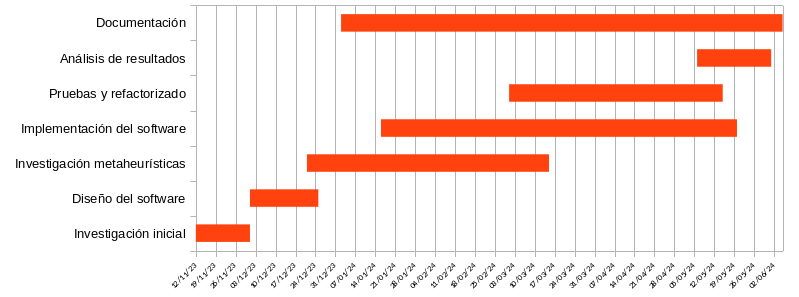
\includegraphics[width=0.8\textwidth]{imagenes/chapter2/gantt-fin.png}
        \caption{Diagrama de Gantt}
    \end{figure}
\end{frame}

\begin{frame}
    \frametitle{Presupuesto}
    \begin{columns}
        \column{1\textwidth}
        \begin{itemize}
            \item \textbf{Sueldo}: $25$€/hora, $340$ horas, total $8.500$€.
            \item \textbf{Portátil}: HP Pavilion, $1000$€, usado $8$ meses, costo $133.3$€.
            \item \textbf{Servidor}: Uso del servidor \textbf{Hércules}, costo real cero. Estimación en \textit{Google Cloud}.
        \end{itemize}
    \end{columns}
\end{frame}

\note{

}

\begin{frame}
    \frametitle{Presupuesto}
    \begin{columns}
        \column{1\textwidth}
        \begin{table}[htp]
            \centering
            \begin{tabular}{|l|r|}
                \hline
                \textbf{Item}                    & \textbf{Costo (€)} \\ \hline
                Salario                          & 8500               \\
                Ordenador portátil               & 133.3              \\
                Servidor CPU - GC Compute Engine & 75.84              \\
                \textbf{Total}                   & \textbf{8709.14}   \\ \hline
            \end{tabular}
            \caption{Costo estimado del proyecto}
        \end{table}
    \end{columns}
\end{frame}